\documentclass[english,a4paper,oneside]{article}
\usepackage{babel}	
\usepackage{amsmath}
\usepackage{amssymb}
\usepackage{mathrsfs}
\usepackage{mathtools}
\usepackage[utf8]{inputenc}
\usepackage[T1]{fontenc}	
\usepackage{graphicx}		
\usepackage{dcolumn}		
\usepackage{booktabs}		
\usepackage{eurosym}
\usepackage{siunitx}
\usepackage{amsthm}
%\usepackage{algorithm}
%\usepackage{algpseudocode}
\usepackage{verbatim}
\usepackage{natbib}
%\usepackage{minted} % Code typesetting
\usepackage{multirow}
\usepackage{blkarray} %Block matrix display
\usepackage{todonotes}
\usepackage{cleveref}
\usepackage{caption}
\usepackage{listings}
%\usepackage{fullpage}
\usepackage{marginnote}
\usepackage[top=1.5cm, bottom=1.5cm, outer=5cm, inner=2cm, heightrounded, marginparwidth=2.5cm, marginparsep=2cm]{geometry}

\newcommand{\element}[3]{$^{#2}_{#3}\mathrm{#1}$}
\newcommand\up[1]{\ensuremath{\textup{#1}}}
\newcommand\dd{\ensuremath{\textup{d}}}
\newcommand{\avg}[1]{\left< #1 \right>}
\newcommand{\Var}[1]{\up{Var}}
\DeclareMathOperator{\erf}{erf}

\newtheorem{mytheorem}{Theorem}
\newtheorem{mydefinition}{Definition}


%%%%%
%  GAMS Markup in listings enviroment
%%%%%

\lstdefinelanguage{GAMS}{
morekeywords={
ABORT, ACRONYM, ACRONYMS, ALIAS, ALL, AND, ASSIGN, BINARY, CARD, DISPLAY, EPS, EQ, EQUATION, EQUATIONS, GE, GT, INF, INTEGER, LE, LOOP, LT, MAXIMIZING, MINIMIZING, MODEL, MODELS, NA, NE, NEGATIVE, NOT, OPTION, OPTIONS, OR, ORD, PARAMETER, PARAMETERS, POSITIVE, PROD, SCALAR, SCALARS, SET, SETS, SMAX, SMIN, SOS1, SOS2, SUM, SYSTEM, TABLE, USING, VARIABLE, VARIABLES, XOR, YES, REPEAT, UNTIL, WHILE, IF, THEN, ELSE, SEMICONT, SEMIINT, FILE, FILES, PUT, PUTPAGE, PUTTL, PUTCLOSE, FREE, NO, SOLVE, FOR, ELSEIF, ABS, ARCTAN, CEIL, COS, ERROR, EXP, FLOOR, LOG, LOG10, MAP, MAPVAL, MAX, MIN, MOD, NORMAL, POWER, ROUND, SIGN, SIN, SQR, SQRT, TRUNC, UNIFORM, LO, UP, FX, SCALE, PRIOR, PC, PS, PW, TM, BM, CASE, DATE, IFILE, OFILE, PAGE, RDATE, RFILE, RTIME, SFILE, TIME, TITLE, TS, TL, TE, TF, LJ, NJ, SJ, TJ, LW, NW, SW, TW, ND, NR, NZ, CC, HDCC, TLCC, LL, HDLL, TLLL, LP, WS, /,PROD: },
sensitive = false,
morecomment=[f]*,%
morecomment=[s]{\$ontext}{\$offtext},
%morecomment=[s][\color{green}]{/}{/},
morestring=[b]“,
morestring=[b]‘
}
\lstset{
basicstyle=\fontfamily{pcr}\fontseries{m}\selectfont\footnotesize,
commentstyle=\color{gray}\itshape,
keywordstyle=\color{blue}\bfseries,
stringstyle=\color[rgb]{0.5,0,0.5}\itshape,
showstringspaces=false,
numbers=left,
numberstyle=\color[rgb]{0,0.5,0.5}\fontfamily{pcr}\fontseries{m}\selectfont\tiny,
numberblanklines=false,
showlines=false,
belowskip=\bigskipamount{},
breaklines=true,
%stepnumber=2,
tabsize=6,
%extendedchars=true,
%float=h,
frame=tb
}


\raggedbottom{}
%\parindent = 0pt

\begin{document}

\title{Exam Project 1: Asset Liability Management in a pension fund}
\author{Tue Vissing Jensen, DTU Elektro\footnote{tvjens@elektro.dtu.dk}
		\and Tiago Soares, DTU Elektro\footnote{tiasoar@elektro.dtu.dk}}
\date{\today}
\maketitle

\section{Nomenclature}
\begin{description}
\item[$t \in T = {0, \ldots, \tau}$]{Time steps, measured relative to current year.}
\item[$i \in E$]{ETF index}
\item[$m \in M$]{Months subset index of $T$}
\item[$T_m \subset T$]{Specified interval dates}
\item[$s \in \Omega$]{Scenarios index}
\item[$st \in ST$]{Index over weeks included in monthly scenarios}
\item[$P_{i,t}$]{Price of ETF $i$ at time $t$}
\end{description}



\section{Data download and clustering analysis}

Price data on the ETFs is downloaded from Google Finance using the data download functionality built in to the Pandas module for Python.
We use the closing price of the ETF for each day to represent the day's price.
Any ETF with less than 2400 data points is excluded, leaving 93 of the initial 100 ETFs to use for further processing.

To cluster the data, it is necessary to define a distance between assets. We compute the correlation coefficient $C_{ij}$ between assets $i$ and $j$, and define the distance between them as
\begin{gather}
d(i,j) = 1 - C_{ij}^2  \in [0, 1].
\end{gather}
This distance will tend to group together assets that are more correlated and/or anti-correlated together.
This is intuitively a reasonable measure, as (1) going long on an asset is the same as going short on an asset that is anti-correlated with it, and we wish to treat short and long assets the same in this analysis, and (2) the difference between a correlation of 1.00 and 0.95 is more significant than between 0.05 and 0.00.


\begin{figure}[tp]
\centering
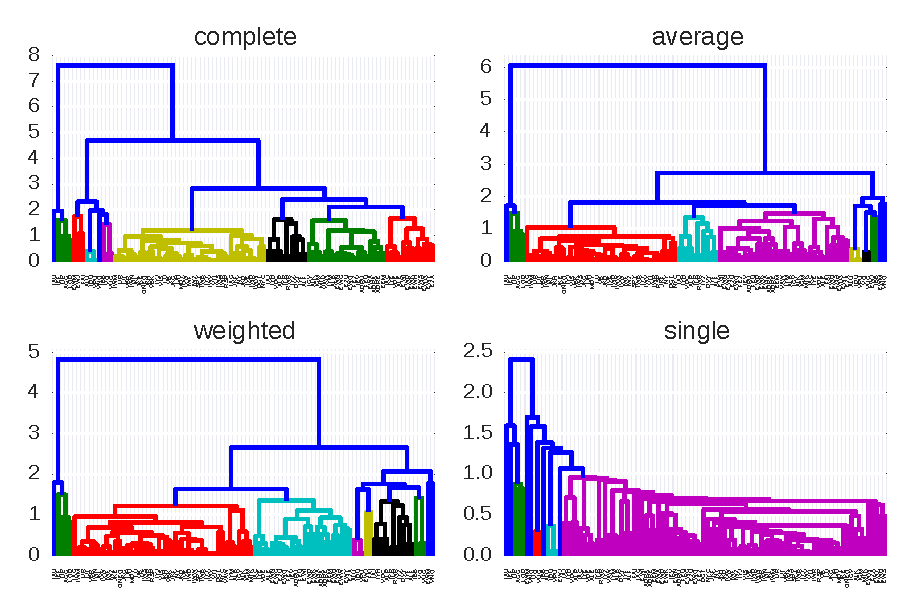
\includegraphics{pic/dendro_methods.pdf}
\caption{DELETE ME IN FINAL:\ Dendrogram of clustering found by various methods. All non-blue leaves are trimmed by the max-mean and the min-std criteria.}
\label{fig:bondsyield}
\end{figure}

\begin{figure}[tp]
\centering
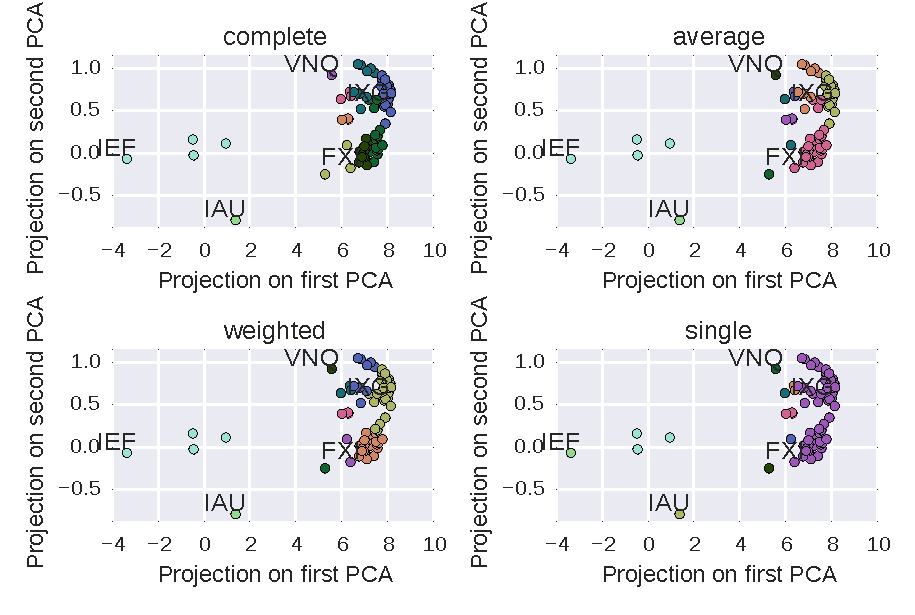
\includegraphics{pic/pca_methods.pdf}
\caption{Projection of asset correlation onto the largest principal components. These account for 78.58\% and 4.51\% of the variance, respectively.}
\label{fig:bondsyield}
\end{figure}


\section{Scenario generation}

The period of study considered in this work is  between 02/02/2005 and 12/11/2014, with the aim to produce a back-test starting on 27/02/2008.
In order to generate scenarios to be used for CVaR model, several assumptions are needed. The historical return for each ETF over the period $t$ is given by
\begin{gather}
r_{i,t} = \frac{P_{i,t+1}}{P_{i,t}}-1, \;\; \forall i \in E, t \in T
\end{gather}
The scenarios are randomly generated picking four dates in a specified interval and taking the historical returns for the ETF's as
\begin{gather}
WRS_{i,st,s,m} = r_{i,t}  \up{ for } t \equiv RANDOM(T_{m}), \;\; \forall i \in E, st \in ST, s \in \Omega, m \in M
\end{gather}
where $WRS_{i,st,s,m}$ is the weekly return scenarios for each month $m$.
The first specified interval$T_1$ where is picked the historical returns is between 28/01/2005 and 27/02/2008.
For each $m$ the specified interval shift itself one month until the end of the period of study (12/11/2014).
The monthly return for each of scenario $MRS_{i,s,m}$ is based on accumulating the four weeks return scenario and is determined as
\begin{gather}
MRS_{i,s,m} = \prod_{st} (1+WRS_{i,st,s,m}) -1, \;\; \forall i \in E, s \in \Omega, m \in M
\end{gather}


\section{CVaR model}\label{sec:CVaR}

The CVaR model was built based on the first set of scenarios with start date 2008-02-27, obtained from scenario generaion chapter. Based on this set is determined the value and expected value of each ETF $i$, for each scenario $s$. In addition, is considered a initial budget of 1 million kr. The CVaR model is defined as
\begin{align}
\sum_{i} x_{i} &= \up{Budget} \\
\up{MeanReturn} &\ge \mu_{\up{Target}} \up{Budget} \\
\up{VaRDev}_{s} &\ge \up{Losses}_{s} - \up{VaR} \; \; \forall s \\
\up{Losses}_{s} &= \sum_{i} x_{i} - \sum_{i} \up{P}_{i,s} x_{i} \; \; \forall s \\
\up{CVaR} &= \up{VaR} + \frac{1} {1 - \alpha} \sum_{s} \up{pr}_{s} \up{VaRDev}_{s} \\
\up{MeanReturn} &= \sum_{i} \up{EP}_{i} x_{i}
\end{align}
where $ \mu_{\up{Target}}$ is 0, $\up{P}_{i,s}$ is the value of each ETF $i$ by scenario $s$, $\up{pr}_{s}$ is the probability of each scenario $s$ and is assumed to be linearly distributed over the scenarios, $\up{EP}_{i}$ is the expected value for each ETF $i$, and $\alpha$ is assumed to be 0.5.
In order to obtain the efficient frontier based on 10 optimal solutions of CVaR model is neccesary to find the minimum CVaR solution, as well as the CVaR solution related to the maximum possible return. Minimizing the model in order to CVaR variable, it returns the minimum CVaR solution of efficient frontier. Maximizing the model in order to MeanReturn variable, it returns the CVaR solution for the maximum average return. Based on this extreme points, a linear $\up{CVaR}_{\up{Target}}$ is created for the 10 runs. A constraint for limit the space solution movement to the $\up{CVaR}_{\up{Target}}$ is included in the CVaR model, and is defined as
\begin{align}
\up{CVaR} &\le \up{CVaR}_{\up{Target}} 
\end{align}
For each of the 10 runs, the CVaR model is optimized in order to maximize the MeanReturn variable. The efficient frontier of the 10 optimal solutions is presented in Figure~\ref{fig:frontier}. 






A CVaR bound of 0.0 indicates that CVaR is minimal, with 1.0 indicating that the optimization solely considers mean return.


\begin{figure}[tp]
\centering
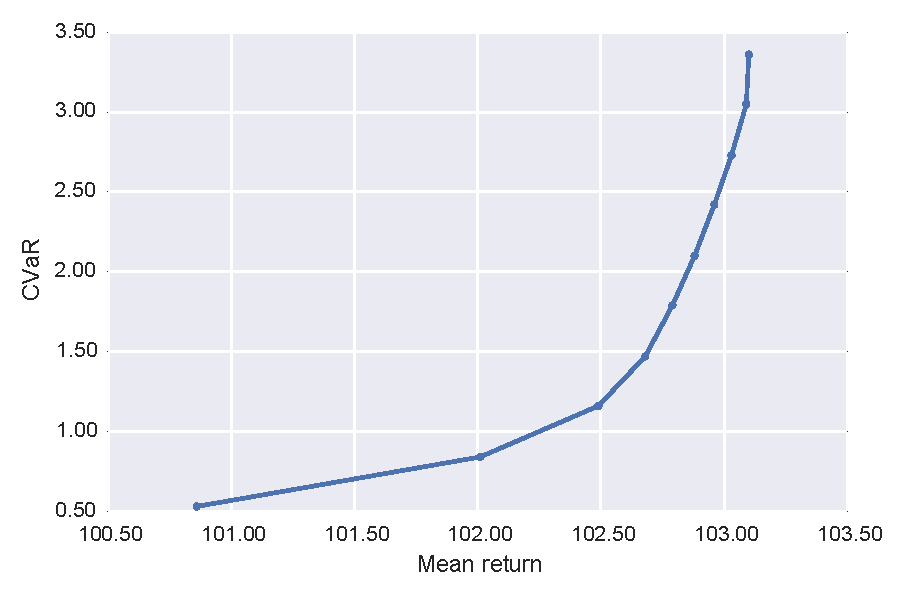
\includegraphics{../pic/frontier.pdf}
\caption{Optimal frontier for equidistant steps in CVaR.}
\label{fig:frontier}
\end{figure}

\begin{figure}[tp]
\centering
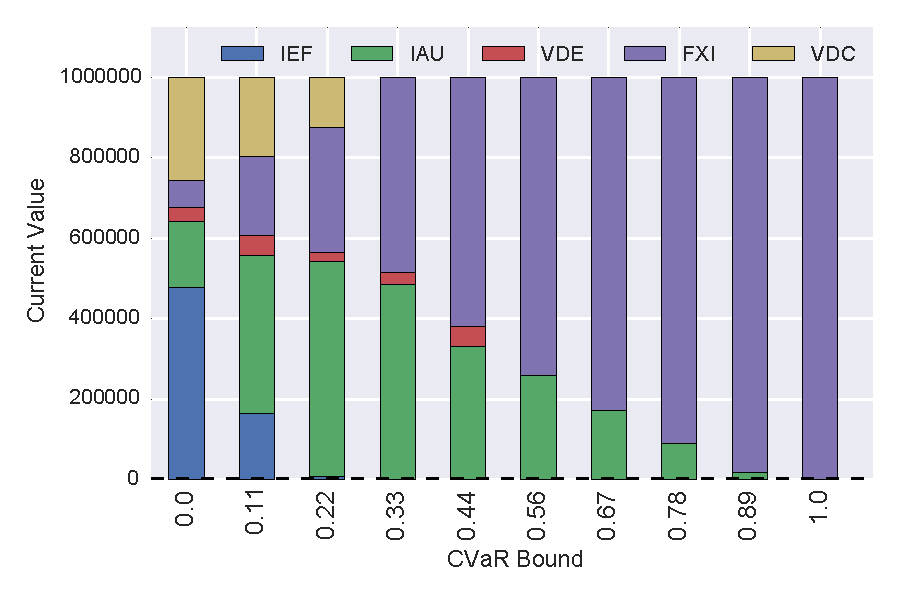
\includegraphics{../pic/Stake_vs_CVaR.pdf}
\caption{Portfolios at varying levels of the CVaR bound.}
\label{fig:scenarioreturn}
\end{figure}

\begin{figure}[tp]
\centering
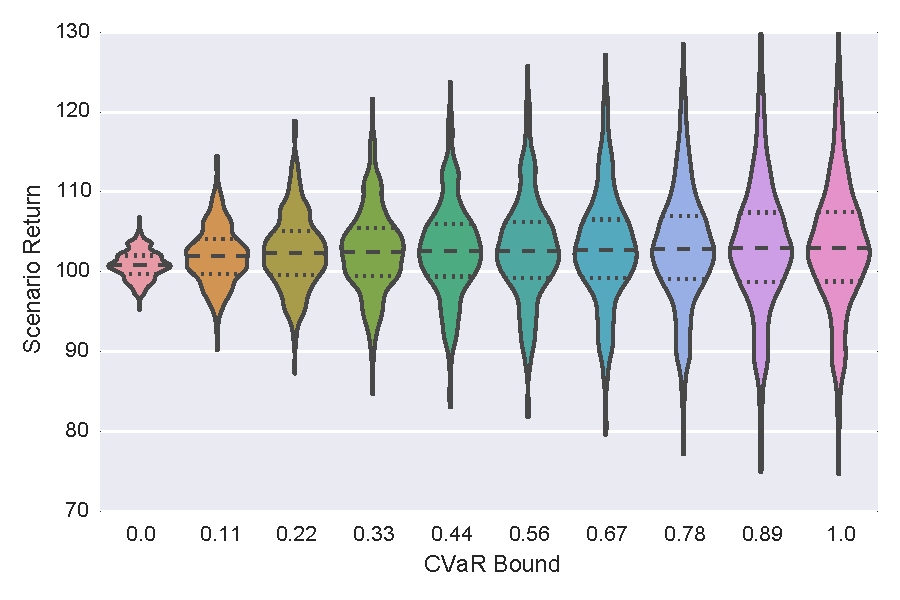
\includegraphics{../pic/Scenario_Return.pdf}
\caption{Scenario return for portfolios at varying levels of the CVaR bound.
The distributions for each bound are mirrored on the vertical axis, with the mean (dashed) and standard deviation (dotted) shown.}
\label{fig:scenarioreturn}
\end{figure}

Figure~\ref{fig:scenarioreturn} compares the scenario return at varying levels of the CVaR bound.

\section{Portfolio revision implementation}
The portfolio revision model is an extension of the CVaR model to revise and evaluate portfolios after some time has past.
In this work, is assumed that four weeks are gone and the previous portfolio on section~\ref{sec:CVaR} could no longer be credible and acceptable.
So, a revision of the portfolio on the (2008-03-28) to maximize the return under two different strategies (risk averse and risk neutral) are considered.
The portfolio revision entails some costs for the transactions deviations on the portfolio.
Here, we assume a transaction cost of 0.1\% of the traded amount in kr., and a minimum cost of at least 50 kr per trade.
These costs are taken to be paid from our own pocket outside of the value of the assets.

The portfolio revision model is defined as
\begin{align}
\up{TotalCost} &= \lambda \up{CVaR} - {\left( 1 - \lambda \right)} \up{MeanReturn} + \up{TradeCost} \\
x^\up{old}_{i} + x^\up{difference}_{i} &= x_{i} \; \; \forall i \\
\sum_{i} x^\up{old}_{i} &= \sum_{i} x_{i} \\
x^\up{difference}_{i} &\le B_{i} \up{M} \; \; \forall i \\
-x^\up{difference}_{i} &\le B_{i} \up{M} \; \; \forall i \\
\up{TradeCost} &= \sum_{i} \up{TC}_{i} \\
\up{TC}_{i} &\ge B_{i} \up{penalty} \; \; \forall i \\
\up{TC}_{i} &\ge 0.001 x^\up{difference}_{i} \; \; \forall i \\
\up{TC}_{i} &\ge - 0.001 x^\up{difference}_{i} \; \; \forall i 
\end{align}
where $\lambda$ is the level of risk of the strategy (1 - Risk Averse ; 0 - Risk Neutral), TradeCost is the total cost of the trades of all changes in portfolio, and $x^\up{old}_{i}$ is the previous result of portfolio updated with the current historical monthly return.
In this way, the first $x^\up{old}_{i}$ is based on the results of section~\ref{sec:CVaR} using the risk averse result.
The difference between the $x^\up{old}_{i}$ and the new $x_{i}$ is given by $x^\up{difference}_{i}$.
$B_{i}$ is a binary variable which characterizes if there is or is not a transacation in each ETF $i$, and M is a high constant value to allow the selection of trade or not trade, chosen here to be equal to the value of the portfolio.
$\up{TC}_{i}$ is the trade cost incurred due to trading in each ETF $i$, and penalty corresponds to the trade cost of 50 kr.
In addition to the previous constraints, constraints~\eqref{eq:MeanReturn}~through~\eqref{eq:VarDev} in the CVaR model presented in section~\ref{sec:CVaR} is considered as constraints in the portfolio revision model.

The initial solution is obtained running the full portfolio revision mode where the value of $x^\up{old}_{i}$  is based on the previous results of CVaR model updating with the current historical return (2008-03-26). 
$x^\up{old}_{i}$  is given by
\begin{align}
x^\up{old}_{i} &= x_{i} (1+ r_{i,m})
\end{align}
where $r_{i,m}$ is the histoical monthly return.

\begin{figure}[tpbh]
\centering
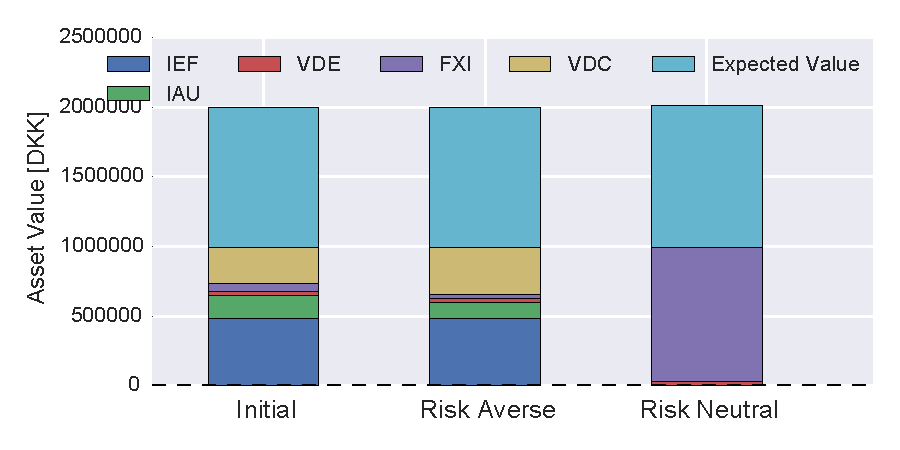
\includegraphics[width=1.0\textwidth]{../pic/portfoliorevision_portfolio.pdf}
\caption{Initial portfolio versus those found by the two types of traders.}
\label{fig:prevpf}
\end{figure}

\begin{table}
\caption{Stats for portfolios found by portfolio revision model.}\label{tbl:portfoliotabel}
\centering
\begin{tabular}{lrrr}
\toprule
{} &  Expected Profit &      CVaR &  Trading Cost \\
\midrule
Type         &                  &           &               \\
Initial      &          8423.76 &   3436.86 &          0.00 \\
Risk Averse  &          6545.42 &   2469.89 &        214.37 \\
Risk Neutral &         24735.63 &  36958.75 &       1820.37 \\
\bottomrule
\end{tabular}

\end{table}

The aim of the present section is to minimize the TotalCost of the full portfolio revision model for each type of strategy (risk averse and risk neutral).
The portfolios are shown on Figure~\ref{fig:prevpf}, while the resulting expected value, CVaR and trading are presented in Table~\ref{tbl:portfoliotabel} considering a comparison between the different strategies and the initial solution. 

The risk-averse strategy makes a small adjustment to the portfolio to decrease the CVaR, while the risk-neutral trader throws away pretty much the entire portfolio to nearly only include a single, high risk asset with high historic return.
Trading a very large value in this way yields a very high trading cost, which is made up for by the large increase in expected profit.

\section{Back-test results}

The implementation of back-test results is based on running the portfolio revision model for each month until the last portfolio revision at 2014-06-18.
The portfolio revision model is performed for each month, where $x^\up{old}_{i}$ is updated every run, with the previous portfolio updated with the historical month return of the current month.
I.e. $x_i^\up{old} \leftarrow (1 + HMR_{i,m}) * x_i$.

\begin{figure}[tpb]
\centering
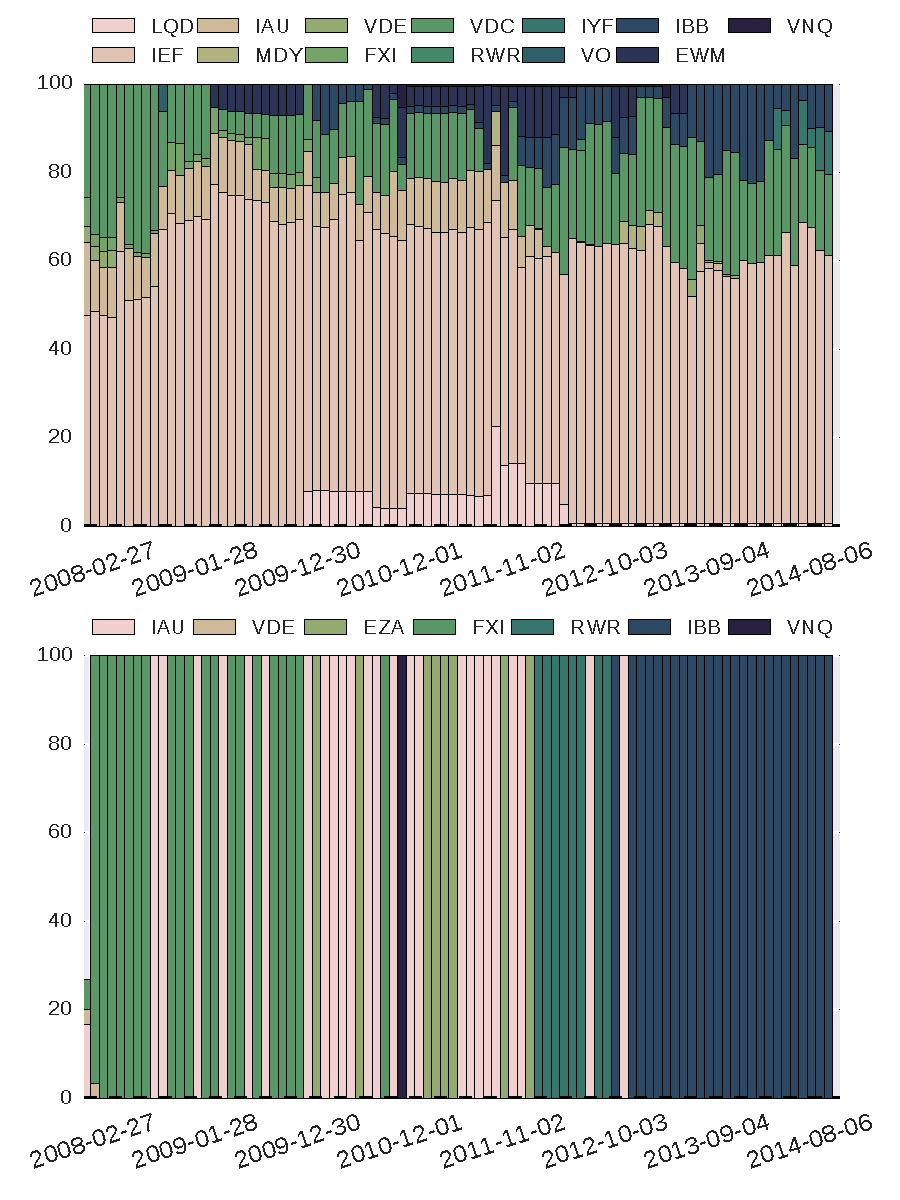
\includegraphics{../pic/trading_portfolio.pdf}
\caption{Portfolios found by the risk-averse (top) and risk-neutral (bottom) trading strategies.}
\label{fig:tradingportfolios}
\end{figure}

The optimal portfolio mix for each period considering all its revision for both risk averse and risk neutral strategies are illustrated in Figure~\ref{fig:tradingportfolios}.
The risk averse strategy always obtain a mixed portfolio in order to minimize the risk of bad return.
One can verify that the IAU assets is in general the base of the portfolio mix for risk averse strategy.
Looking at the risk neutral strategy, on the other hand, it tries to bank on the single asset with the largest expected return.
At early times, the FXI asset has high participation, since that ETF has an upward tendency until the crash. After the crash, IAU has a very good upward tendency.
At this point IBB start slowly a upward tendency, which is more steeper in later periods.
In this way and based on the behaviour of the ETFs in Figure~\ref{fig:prices_selected}, the portfolio revision obtained for both perspectives is as expected.

\begin{figure}[tpb]
\centering
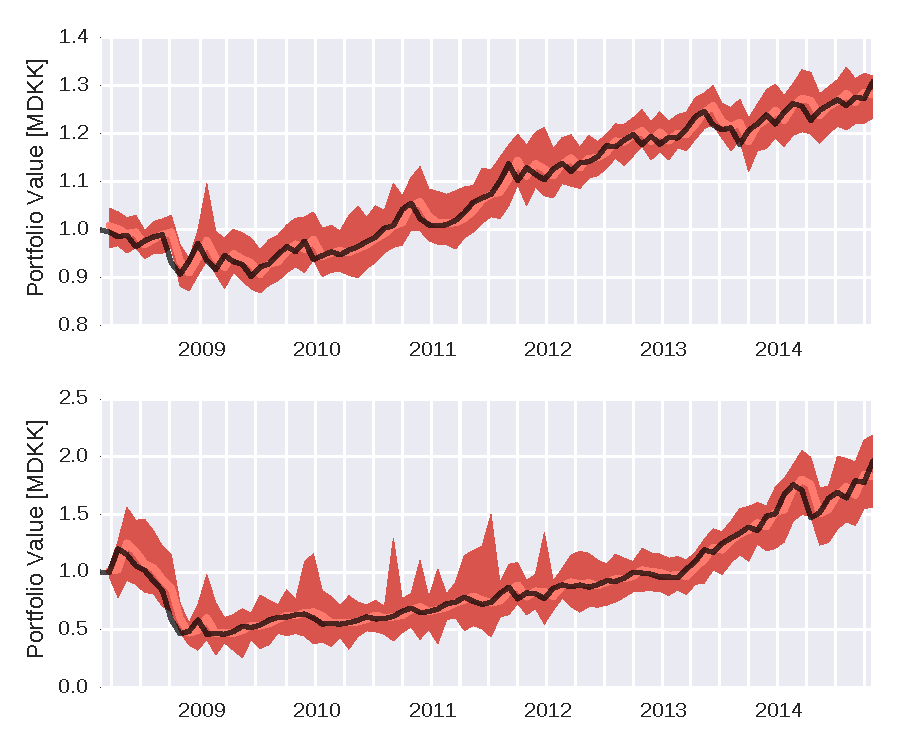
\includegraphics{../pic/trading_forecasted_value.pdf}
\caption{Nominal values of portfolios over time (Black line) versus forecasted mean value (light red). The shaded region indicates the maximum and minimum forecasted values of the ensembles. The risk avers (top) and risk neutral (bottom) strategies for portfolio valueare considered.}
\label{fig:tradingforecastedvalues}
\end{figure}

The historical values of the portfolios found is compared to that forecasted by the scenarios of the previous trading period in Figure~\ref{fig:tradingforecastedvalues}.
The forecasted values always seem to trail the actual values by 1 month.
This is explained as the result of the forecast essentially being a persistence forecast due to the small average return provided.

Looking at the spread the scenarios reveal that only in a few cases around mid-late-2008 do the returns fall outside the interval predicted by the forecast, indicating that the scenarios are able to capture the risk in the market, despite missing the movement of the portfolio mean.

\begin{figure}[tpb]
\centering
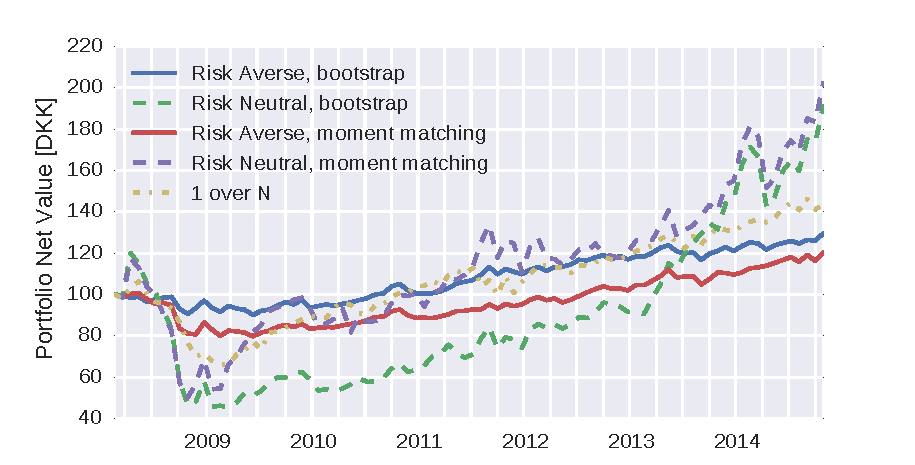
\includegraphics{../pic/trading_portfolio_value.pdf}
\caption{Net values of portfolios over time. (Net value = nominal value minus cumulative trading costs)}
\label{fig:tradingportfoliovalues}
\end{figure}


% TODO: REWRITE

The portfolio value over the time for each of the strategies is presented in Figure~\ref{fig:tradingportfoliovalues}.
One can see that different strategies has different average behaviours, as well as the worst and best case of the scenarios.
The risk neutral strategy is the strategy that achieves higher return in the end of the period of investment. 
However, it does not mean that is the best strategy among all periods.
On average, the ideal strategy throughout the time is the use of both strategies to maximize the expected return.
In the early six months is advised the use of risk neutral strategy.
Than risk averse should be used until the early months of 2013.
In the remaining months, risk neutral ensures more return to the investor.

Regarding the results of portfolio revision model considering the scenario generation of moment matching, we conclude that the patterns of the results are very similar.

To compare the strategies with a simple trading scheme, the $1/N$ strategy is used; on the first trading day we invest an equal amount into each asset, and then leave the assets be for the entire trading period.
In order to compare a 1/N strategy with the strategy results of risk averse and risk neutral is presented the Figure~\ref{fig:tradingportfoliovalues}.
Furthermore, is considered the results of each strategy (risk averse and risk neutral) for each scenario generation method (bootstrap and moment matching).

One can see that the risk averse strategy from the bootstrap method present on average higher portfolio value than the same strategy but based on moment matching method.
On the other hand, risk neutral strategy from moment matching strategy presents on average higher portfolio values than the strategy based on bootstrap method.
Regarding to the 1/N strategy, one can identify that is a strategy that returns a stable portfolio value throughout the periods.
However, is a strategy that presents results between the two extreme strategies (risk averse and risk neutral).
In the end, is expected a higher return value on risk averse strategy, and the lower return value on risk neutral strategy.

% Until here

\begin{table}[tpb]
\caption{Comparison of trading strategies}\label{tbl:strategytabel}
\centering
\begin{tabular}{lrrrl}
\toprule
{} & Final Nominal &  Trading &  Final Net & Annualized \\
{} & Value & Costs & Profit & Return \\
\midrule
Risk Averse, bootstrap        &              1259714 &          10810 &            248904 &             3.6 \% \\
Risk Neutral, bootstrap       &              1639882 &          43283 &            596599 &             7.7 \% \\
Risk Averse, moment matching  &              1172530 &           5797 &            166733 &             2.5 \% \\
Risk Neutral, moment matching &              1701345 &           8787 &            692558 &             8.7 \% \\
1 over N                      &              1462676 &              0 &            462676 &             6.2 \% \\
\bottomrule
\end{tabular}

\end{table}


A comparison between the final numbers of the trading strategies is shown in Table~\ref{tbl:strategytabel}.
Four things are noteworthy here:

Firstly, the highest return for the risk averse strategies is found by the boostrap scenarios rather than the moment matching ones, whereas they perform oppositely for the risk neutral strategy.
This is reasonable, as the risk averse strategy is sensitive to correlations in the data, which are destroyed by the moment matching scenarios, while the risk-neutral strategy needs an accurate representation of the mean, which is captured more closely by the moment matching scenarios.

Secondly, the trading costs are much higher for the bootstrap scenarios than for the moment matching scenarios.
This may be understood as the bootstrap scenarios can change quite a lot over time, while the moment matching scenarios will tend to jump around less in between time steps.

Thirdly, the trading costs are higher for the risk neutral strategy than for the risk averse strategy. This is due to the risk neutral strategy constantly throwing away the entire portfolio as shown on Figure~\ref{fig:tradingportfolios}.

Fourthly, the 1 over N strategy manages to outperform both risk averse strategies, and would have outperformed the risk neutral strategies as well if the market hadn't experienced a steady upswing in 2013 and 2014.

As a closing remark, taking the old advice to just bet on gold, and invest everything in IAU, cashing out in 2012 would have given an annualized return across the period of $9.4 \%$. If this money had then been reinvested in IBB, the annualized return would have been $\sim 27 \%$.
In other words, clairvoyance outperforms any mortal strategy.

\section{Scenario generation via moment matching}

For the moment matching scenarios, we are looking to match the mean, variance, skewness and kurtosis with historical data.
Calculating these for each month $m$ as
\begin{gather}
\mu_{m,i} = \frac{1}{|T_m|} \sum_{t \in T_m} r^m_{i,t} \\
\beta_{m,i} = \frac{1}{|T_m|} \sum_{t \in T_m} {\left( r^m_{i,t} - \mu_{m,i} \right)}^2 \\
\gamma_{m,i} = \frac{1}{|T_m|} \sum_{t \in T_m} {\left( r^m_{i,t} - \mu_{m,i} \right)}^3 \\
\eta_{m,i} = \frac{1}{|T_m|} \sum_{t \in T_m} {\left( r^m_{i,t} - \mu_{m,i} \right)}^4 ,
\end{gather}

we solve the following optimization problem to find the scenario sets ${\{\xi_{i,s}\}}_{m}$:

\begin{align}
\min \sum_i \left(
	{(\tilde{\mu}_i - \mu_{m,i})}^2 +
	{\left( \frac{\tilde{\beta}_i}{\beta_{m,i}} - 1 \right)}^2 +
	{\left( \frac{\tilde{\gamma}_i - \gamma_{m,i}}{\beta_{m,i}^{3/2}} \right)}^2 +
	{\left( \frac{\tilde{\eta}_i - \eta_{m,i}}{\beta_{m,i}^{2}} \right)}^2
\right)
\label{eq:momentobj}
\end{align}
S.t.
\begin{align}
\tilde{\mu}_i &= \frac{1}{|\Omega|} \sum_{s \in \Omega} \xi_{i,s} \\
\tilde{\beta}_i &= \frac{1}{|\Omega|} \sum_{s \in \Omega} {\left( \xi_{i,s} - \tilde{\mu}_i \right)}^2 \\
\tilde{\gamma}_i &= \frac{1}{|\Omega|} \sum_{s \in \Omega} {\left( \xi_{i,s} - \tilde{\mu}_i \right)}^3 \\
\tilde{\eta}_i &= \frac{1}{|\Omega|} \sum_{s \in \Omega} {\left( \xi_{i,s} - \tilde{\mu}_i \right)}^4
\end{align}

The normalization in~\eqref{eq:momentobj} by powers of $\beta_{m,i}$ ensures that the objective is scale-invariant, and that each term has an equal weight.


\clearpage

\appendix

\section{Gams code\label{sec:appendixcode}}

All code from this project is available at \url{www.github.com/TueVJ/OptFinFinalExam}~.

\end{document}

